\documentclass[a4paper,11pt,twoside,openright]{report}

\usepackage{graphicx}
%\usepackage{ngerman}
\usepackage[utf8x]{inputenc}
\usepackage{fancyvrb}
\usepackage{courier}
\usepackage{helvet}
\usepackage{tikz}
\usepackage{xcolor}
\usepackage{pdfpages}
\usepackage[strict]{changepage}
\usepackage{wrapfig}
\usepackage{color}
\usepackage{amssymb}% http://ctan.org/pkg/amssymb
\usepackage{pifont}% http://ctan.org/pkg/pifont
\usepackage{tikz}
\usepackage{url}
\usepackage{caption}
\usepackage{subcaption}
\usetikzlibrary{shapes,arrows}
\usepackage{xcolor}
\usepackage{multirow}
\usepackage{rotating}

\usepackage{hyperref}


% styles for flowcharts
\tikzset{vertex/.style = {shape=circle,draw,minimum size=1.5em}}
\tikzset{edge/.style = {->,> = latex'}}
\tikzstyle{block} = [rectangle, draw, text width=20em, text centered, rounded corners, minimum height=0.75em]


\pdfoptionpdfminorversion=6

% \definecolor{se_dark_blue}{RGB}{0,103,166} % powerpoint
\definecolor{se_dark_blue}{RGB}{0,96,178} % website
% \definecolor{se_light_blue}{RGB}{119,158,201} % powerpoint
\definecolor{se_light_blue}{RGB}{129,160,225} % website


%% setup listings
\usepackage{listings}
\lstset{
    numbers=left,
    numberstyle=\tiny,
    numbersep=5pt,
    xleftmargin=11pt,
    xrightmargin=4pt,
    frame=single,
    aboveskip=0pt,
    belowskip=-6pt,
    sensitive=true,
    float=!t,
    breaklines=false,
    captionpos=b,
    tabsize=2,
    showstringspaces=false,
    basicstyle=\small\ttfamily,
    morecomment=[l]{//},
    morecomment=[s][\itshape]{/**}{*/}
}

%% defines the listings laguage named 'MontiArc' derived from the language 'Java' 
%% adding the below listed keywords. See 
%% ftp://ftp.tex.ac.uk/tex-archive/macros/latex/contrib/listings/listings.pdf
%% for listings documentation
\lstdefinelanguage{MontiArc}[]{Java}{
  morekeywords={component, port, in, out, inv, package, import, connect, autoconnect}
}

% Seite einrichten
\setlength{\voffset}{-1in}
\setlength{\hoffset}{-1in}

\setlength{\topmargin}{2.5cm}		   
\setlength{\headheight}{0cm}		   
\setlength{\headsep}{0cm}		   
\setlength{\oddsidemargin}{3,3cm}  % innen ein wenig mehr Rand für die Klebebindung
\setlength{\evensidemargin}{2,7cm} % dafür außen ein wenig weniger
\setlength{\textwidth}{15cm}		   
\setlength{\textheight}{23,5cm}		   
\setlength{\parindent}{0cm}

\newcommand{\emptyLine}{{\LARGE ~\\}}

\begin{document}

% Einrücken von Absätzen verhindern und 1.5 Zeilen Absatzabstand
\setlength{\parindent}{0pt}
\setlength{\parskip}{1.5ex plus0.5ex minus0.5ex}

%% Dieses Teildokument beschreibt die Titelseite.
%

% Seitenzähler auf 1, Römische Ziffern.
\setcounter{page}{1}
\pagenumbering{roman}

\thispagestyle{headings}

%\changepage{<text height>}{<text width>}{<even-side margin>}{<odd-side margin>}{<column sep.>}{<topmargin>}{<headheight>}{<headsep>}{<footskip>}
\changepage{5,1cm}{2.4cm}{}{-0.7cm}{}{-2,3cm}{}{}{}

% Eigentliche Titelseite.
\begin{titlepage}
	
\begin{figure}\raggedleft
\includegraphics[height=3.0cm]{src/pic/logo.jpg}\end{figure}
  
\begin{tikzpicture}[overlay]

% horizontal lines
\draw[color=se_dark_blue, thick] (-1.6, 0.9) -- (17.4, 0.9);
\draw[color=se_light_blue, thick] (-1.4, 0.7) -- (17.4, 0.7);

% vertical lines
\draw[color=se_dark_blue, thick] (-1, 0.9) -- (-1, -24.5);
\draw[color=se_light_blue, thick] (-0.8, 0.7) -- (-0.8, -24.5);

\end{tikzpicture}

\vspace*{-1.5em}

\begin{flushleft}
  {\fontfamily{phv}  
  	{\LARGE
      Rheinisch Westfälische Technische Hochschule Aachen \\
      Lehrstuhl für Software Engineering \\}
    \vspace{3em}
  
%    {\LARGE \textbf{Seminararbeit}\\} 
    {\emptyLine}
    {\LARGE \textbf{Feature Location Techniques}\\} 
    {\emptyLine}
    {\emptyLine}
%    {\LARGE \textbf{Dritte Titel-Zeile}\\} % Oder \emptyLine falls nicht Titel kürzer
%    {\LARGE \textbf{Vierte Titel-Zeile}\\} % Oder \emptyLine falls nicht Titel kürzer
    \vspace{3em}
		
    {\Large \textbf{Seminararbeit}\\}
		\vspace{3em} 
		
		{\large von\\} % presented by
    
    {\LARGE \textbf{Bergerbusch, Timo}\\}
    \vspace{3em} 
		    
    {\Large \textbf{1. Prüfer: Prof.\ Dr.\ B.\ Rumpe}\\}
    \vspace{1em} 
    {\Large \textbf{2. Prüfer: Dipl.-Inform.\ C.\ Schulze}\\}
    \vspace{1em} 
    {\Large \textbf{Betreuer: Dipl.-Inform.\ C.\ Schulze}\\}
    \vspace{7em} 

    {\large Diese Arbeit wurde vorgelegt am Lehrstuhl für Software Engineering \\}
    \vspace{1em}
    % The present work was submitted to the chair of software engineering
		{\large	Aachen, den \today\\}
  }
\end{flushleft}

\end{titlepage}

\changepage{-5,1cm}{-2.4cm}{}{0.7cm}{}{2,3cm}{}{}{}





 %Dieses Teildokument beschreibt die Titelseite.
%

% Seitenzähler auf 1, Römische Ziffern.
\setcounter{page}{1}
\pagenumbering{roman}

\thispagestyle{headings}

%\changepage{<text height>}{<text width>}{<even-side margin>}{<odd-side margin>}{<column sep.>}{<topmargin>}{<headheight>}{<headsep>}{<footskip>}
\changepage{5,1cm}{2.4cm}{}{-0.7cm}{}{-2,3cm}{}{}{}

% Eigentliche Titelseite.
\begin{titlepage}
	
\begin{figure}\raggedleft
\includegraphics[height=3.0cm]{src/pic/logo.jpg}\end{figure}
  
\begin{tikzpicture}[overlay]

% horizontal lines
\draw[color=se_dark_blue, thick] (-1.6, 0.9) -- (17.4, 0.9);
\draw[color=se_light_blue, thick] (-1.4, 0.7) -- (17.4, 0.7);

% vertical lines
\draw[color=se_dark_blue, thick] (-1, 0.9) -- (-1, -24.5);
\draw[color=se_light_blue, thick] (-0.8, 0.7) -- (-0.8, -24.5);

\end{tikzpicture}

\vspace*{-1.5em}

\begin{flushleft}
  {\fontfamily{phv}  
  	{\LARGE
      RWTH Aachen University \\
      Software Engineering Group \\}
    \vspace{3em}
  
    %    {\LARGE \textbf{Seminararbeit}\\} 
    {\emptyLine}
    {\LARGE \textbf{Feature Location Techniques}\\} 
    {\emptyLine}
    {\emptyLine}
%    {\LARGE \textbf{Dritte Titel-Zeile}\\} % Oder \emptyLine falls nicht Titel kürzer
%    {\LARGE \textbf{Vierte Titel-Zeile}\\} % Oder \emptyLine falls nicht Titel kürzer
    \vspace{3em}
		
    {\Large \textbf{Seminar Paper}\\}
		\vspace{3em} 
		
		{\large presented by\\} 
    
    {\LARGE \textbf{Bergerbusch, Timo}\\}
    \vspace{3em} 
		    
    {\Large \textbf{1st Examiner: Prof.\ Dr.\ B.\ Rumpe}\\}
    \vspace{1em} 
    {\Large \textbf{2nd Examiner: Dipl.-Inform.\ C.\ Schulze}\\}
    \vspace{1em} 
    {\Large \textbf{Advisor: Dipl.-Inform.\ C.\ Schulze}\\}
    \vspace{7em} 

    {\large The present work was submitted to the Chair of Software Engineering \\}
    \vspace{1em}
    % The present work was submitted to the chair of software engineering
		{\large	Aachen, \today\\}
  }
\end{flushleft}

\end{titlepage}

\changepage{-5,1cm}{-2.4cm}{}{0.7cm}{}{2,3cm}{}{}{}




 % English cover

\clearpage

% Erklaerung

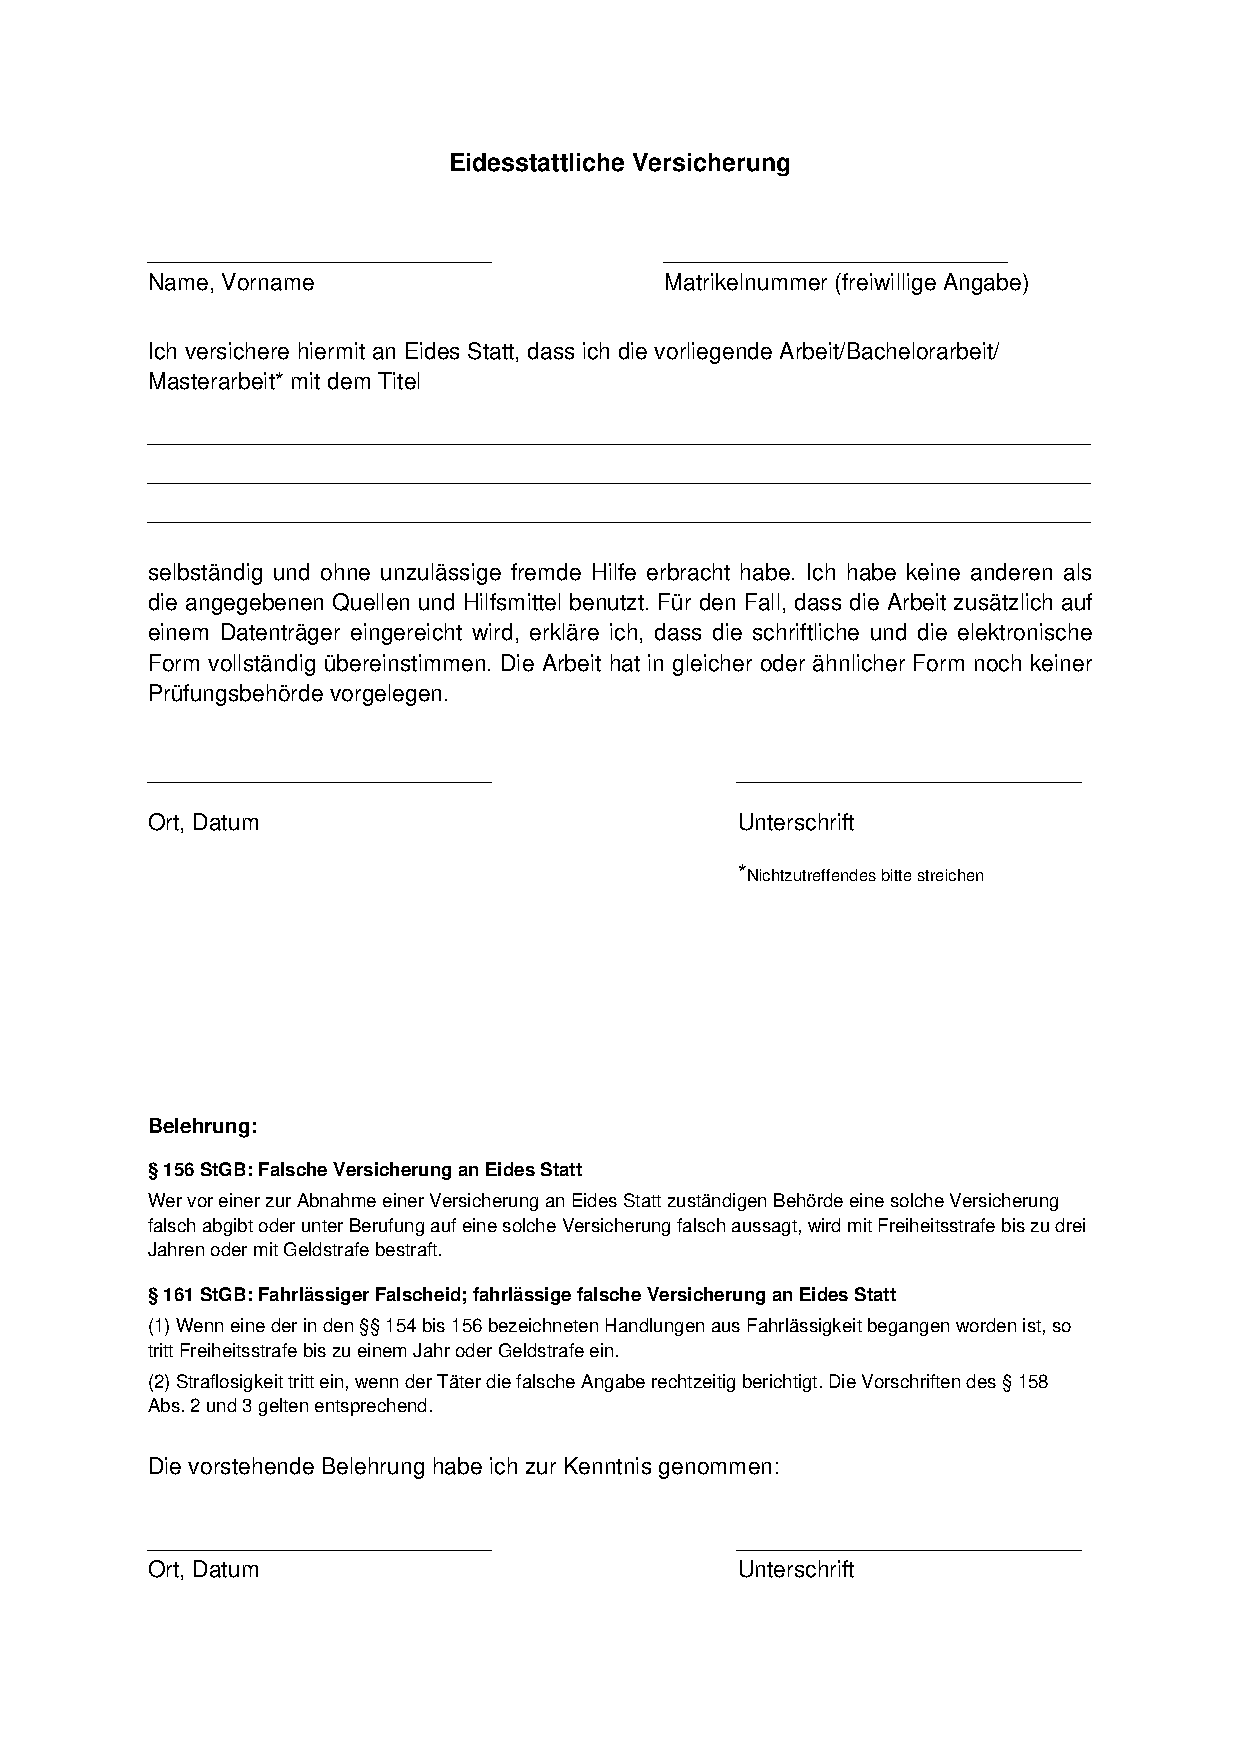
\includepdf[pages={1},offset=-1in -1in]{Formular_Eidesstattliche_Versicherung_neu.pdf}
% \includepdf[pages={1},offset=-1in -1in]{Statutory_Declaration_in_Lieu_of_an_Oath.pdf} % English 

\clearpage

\vspace*{2cm}
% Abstract
%{\bf\Large Kurzfassung} \\ [1em] 
%Eine kurze Zusammenfassung der Arbeit.

%\vspace{10ex}
{\bf\Large Abstract} \\ [1em]
Locating software artefacts that implement a specific program functionality, whether it's functional or non-functional, are called a feature. Detecting features in a program is the main goal of Feature Location Techniques(FLT). It assists software developers during the maintenance and refactoring of the code.
But also the software product line engineering(SPLE), which specifies, designed and implements different products by managing features, uses these techniques to create a product without copying code unstructured but by systematic reuse of the artefacts the FLT's locate \cite{pohl2005software}.

Therefore my seminar paper deals with different feature location techniques from very fundamental methods to some of today's newest research fields. In this paper I introduce a real use case example, to show the real utility of the techniques. The use case will be the location of the \textit{automaticSaveFile}-function of the Freemind mind mapping software, which is an open source mind map editor. \cite{FrM16}.

The beginning of this paper deals with the basics of Feature Location Techniques to understand how techniques are able to define artefacts, the classification of FLT's considering their approach strategy, explaining different techniques of different sets of a taxonomy, regarding their strengths and weaknesses, on a realistic use case of a real software segment. At the end will be a recap of the explained techniques and a forecast about the further development.

\cleardoublepage


%\input{src/tex/aufgabenstellung}

\tableofcontents

\clearpage

% Ab erstem Kapitel Seiten arabisch zählen
\setcounter{page}{1}
\pagenumbering{arabic}

\chapter{Introduction}
%\section{Eins - Eins}
%\subsection{Eins - Eins - Eins}

% Die Logos sind veraltet und duerfen zurzeit nicht verwendet werden!
% Auf Seite \pageref{Logo} in Abbildung \ref{Logo} befindet sich das SE Logo.

A feature location technique is aiming at the locating of software artifacts as a realization of a system requirement. It could be \emph{functional}, like the ability of doing a special kind of computation for example counting elements, or it could be \emph{non-functional} like doing a functional requirement in a given time.
To be able to understand what a feature location technique in detail should be it is necessary to have a basic knowledge about two aspects of modern software engineering. Without either one of the following two underling definitions it's is not clearly definable what a feature location technique should be capable of and there is also no way to rate if a technique is efficient and correct.

On the one hand there a the features. As defined by the Institute of Electrical and electronics Engineers (IEEE) a feature is defined as 'A distinguishing characteristic of a software item (e.g., performance, portability, or functionality)'.\cite{wiki:Softwarefeature} For us simplified a feature is a software artifact implementing a given requirement. Features are often described by the definition of \emph{Rajlich and Chen}, who describe a feature or concept as a triple of \textit{name}, the name of the feature, \textit{intension}, a short precise description, and \textit{extension}, the artifacts implementing the feature.\cite{KR00} \label{Rajlich_Chen}

The the other hand there is the software product line engineering (SPLE). A product line is a variety of products, which in our case are software products, which 'share a common, managed set of features satisfying the specific needs a particular market segment or mission and that are developed from a common set of core assets in a prescribed way.' \cite{SPL}.
A good example are the products of  SAP like the \emph{Business One}, \emph{Business All-In-One} and \emph{Business ByDesign}, which share a basic set of functionality, build up on each other and often are modified to fit the needs of a customer.
The SPLE promotes \textit{systematic}  software reuse being base on the knowledge about the set of available features, relationships among the features and the relationship between features and their artifacts.
The most essential step for unfolding the complexity of existing implementations to be able to transform it into a SPLE includes the identifying of the implemented features and their corresponding artifacts.

This, the locating and defining of a feature, is the problem a feature location technique should solve, so that developers of software product lines are supported during the maintenance and the aspect-/feature oriented refactoring of software. 
%\cleardoublepage


\chapter{Freemind Example}
\label{ch:Freemind Example}

The example used for this paper is the \textit{automatic save file} feature of Freemind, also used in the paper \emph{A Survey of Feature Location Techniques} by \textit{Julia Rubin} and \textit{Marsha Chechik} \cite{rubin2013survey}. Freemind is an open source  mind-mapping tool. The \textit{automatic save file} feature is a good example, because of it's name. Parts of the name are also mentioned in other features, which makes it slightly more difficult to only locate this specific feature.
A related callgraph of the important parts is shown in Fig 2.1.

\begin{wrapfigure}{r}{0.5\textwidth}
  \centering
  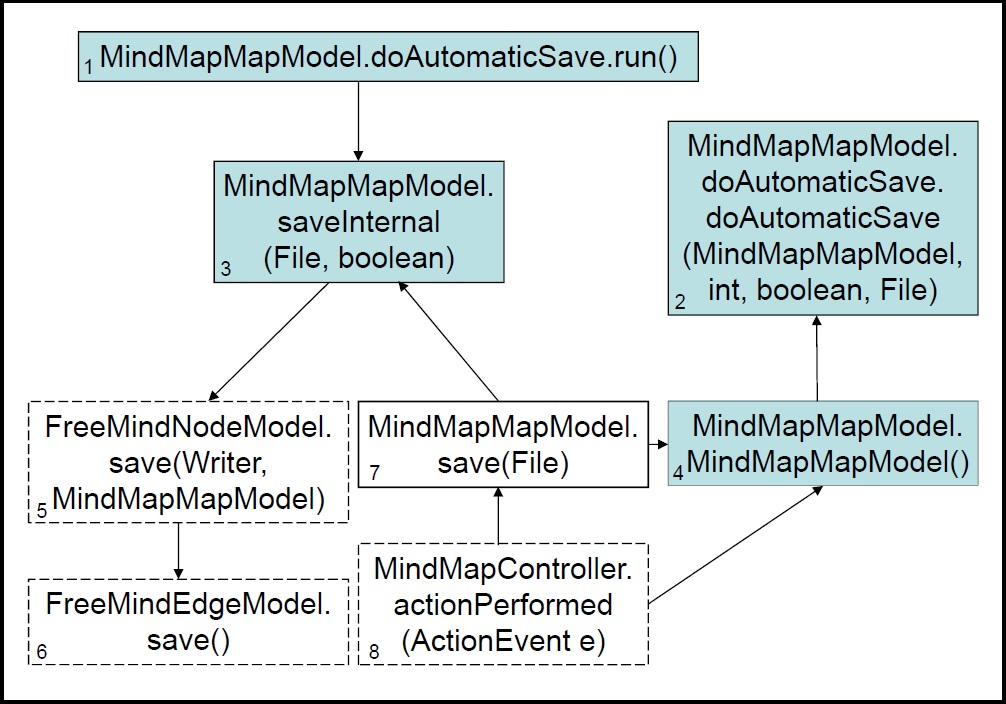
\includegraphics[width=\linewidth]{src/pic/freemind_callgraph}
  \caption{The Freemind callgraph \cite{FrM16} \cite{rubin2013survey}}
  \label{pic:freemind callgraph}
\end{wrapfigure}

In the graph only the relevant constructors and methods are shown and numbered with indices from 1 to 8. These will be further referenced by using the number sign \# and then the corresponding number. Also the feature of the regarded function are highlighted with a blue background colour. These are the methods which should be located if the \emph{automatic save file} function is the wanted feature. Note that all the methods of different classes can in addition call other methods and constructors, which are irrelevant to the feature.
So as it is shown within the graph the feature is mainly implemented by two methods of a subclass of \emph{MindMapMapModel} so called \emph{doAutomaticSave}:
\begin{itemize} 
\item the constructor, which is \#2. This constructor gets a few parameters to configure the \emph{doAutomaticSave}-function and registers the class in the scheduling queue, so that it gets called.
\item the \emph{run()}-function \#1. This Methods gets called after the class is registered in the scheduling queue and everytime a special event occurs. That can be different, like a period of time to schedule an automatic save or a preset number of actions within the main-program. It calls the \emph{saveInternal}-method to do the actual \textit{save}-operation.
\end{itemize}

\newpage
Regarding the previously mentioned definition of a feature by Rajlich and Chen in \autoref{Rajlich_Chen}, the regarded feature can be defined as the following: \newline
\begin{tabular}{ l  l }
  name & \emph{automatic save file}  \\
  intension & saves a file automatically after the occurring of an event\\
 extension & \#1,  \#2, \#3 and \#4\\
\end{tabular} \newline
The methods \#5 to \#8 are not in the extension of the \emph{automaticSaveFile} feature.
Mainly \# 5 and \#6 are called by methods of the \emph{automaticSaveFile} feature, but are not relevant to the specifies of this function.
\#7 and \#8 in fact call \#3 and \#4, but they handle a user triggered save-event, which obviously is not important to the \emph{automaticSaveFile} feature.
\newline \newline
While all feature location techniques try to achieve the same goal, which is locating the matching feature extension to a given feature intension, they differ in the underlying base of assumptions they make to be able to get the traceability. It will be declared more specific in chapter~\ref{ch:Classification and Methodology}. 


\chapter{Basic Underlying Techniques}
\label{ch:basic underlying techniques}

To understand how feature location techniques work it is important to understand a few basic techniques that are commonly used to create or improve feature location. All the basic techniques  will be exemplary executed on the previously introduced Freemind-example in chapter~\ref{ch:Freemind Example}.

\section{Formal Concept Analysis (FCA)}
\label{sec:FCA}
\begin{wrapfigure}[20]{h}{0.5\textwidth}
	\vspace{-1em}
  \centering
  \fbox{
  \begin{tikzpicture}
   % nodes
   \node[block] (a) {$\sigma_1$ = MindMapMapModel.doAutomaticSave.run()};
   \node[block] (b)  [below of=a, node distance = 2 cm] {\color{gray}Mind \color{red}Map \color{blue}Model \color{yellow}do \color{green}Automatic \color{purple}Save \color{orange}run};
   \node[block] (c)  [below of=b, node distance = 2 cm] {\color{gray}mind \color{red}map \color{blue}model \color{yellow}do \color{green}automatic \color{purple}save \color{orange}run};
   \node[table] (d)  [below of=c, node distance = 3.5 cm] {
%		  \begin{center}
		    \begin{tabular}{| l | c |}
		      \hline
		      & $\sigma_1$ \\ \hline
		      \color{gray}mind & \checkmark \\ \hline
		      \color{red}map & \checkmark \\ \hline
		      \color{blue}model & \checkmark \\ \hline
		      \color{yellow}do & \checkmark \\ \hline
		      \color{green}automatic & \checkmark \\ \hline
		      \color{purple}save & \checkmark \\ \hline
		      \color{orange}run & \checkmark \\ \hline
		      \color{black} other &  \\ \hline
		    \end{tabular}
%		  \end{center}
		};

   % edges
   \draw[->] (a) -- node[right] {1. declare every $w_i$} (b);
   \draw[->] (b) -- node[right] {2. decapitalize the $w_i$'s} (c);
   \draw[->] (c) -- node[right] {3. create table} (d);
  \end{tikzpicture}}
  \caption{\#1 of the Freemind Example as example}
  \label{graph:FCA-flowchart}
\end{wrapfigure}
\emph{Formal Concept Analysis} (short: \emph{FCA}) is a predominantly mathematical approach to identify groups of classes and methods compared by the sharing of attributes. The \emph{FCA} regards the binary relation between all objects and attributes and therefore can also provide a model to analyse the hierarchy, because hierarchy structures often have similar relations. \newline
The \emph{FCA}'s goal is to define so called \emph{concepts}. A \emph{concept} is a tuple of extension, the objects that belong to a concept, and intension, all the attributes that \underline{every} object of the extension has.
In order to be able to derive such a \emph{concept} the \emph{FCA} creates an incidence table. The table can be derived in 3 steps as seen in \autoref{graph:FCA-flowchart}:
\begin{enumerate}
  \item declaring every word in the objects and methods as $w_i$ to a new $i$ if the word is not already defined
  \item decapitalizing every $w_i$
  \item creating the table with every decapitalize word as a row and every $\sigma_i$ as a column. The cells $c_{ij}$ are checked if  $\sigma_i$ contains the word $w_i$
\end{enumerate}
\pagebreak
\begin{figure}
	\vspace{-2em}
    \centering
    \begin{tabular}{| l | c | c | c | c | c | c | c | c |}
      \multicolumn{1}{c}{objects} & \multicolumn{1}{c}{$\sigma_1$} & \multicolumn{1}{c}{$\sigma_2$} & \multicolumn{1}{c}{$\sigma_3$} & \multicolumn{1}{c}{$\sigma_4$} & \multicolumn{1}{c}{$\sigma_5$} & \multicolumn{1}{c}{$\sigma_6$} & \multicolumn{1}{c}{$\sigma_7$} & \multicolumn{1}{c}{$\sigma_8$} \\ 
      \multicolumn{1}{c}{$\downarrow$} &  \multicolumn{1}{c}{$\downarrow$} & \multicolumn{1}{c}{$\downarrow$} & \multicolumn{1}{c}{$\downarrow$} & \multicolumn{1}{c}{$\downarrow$} & \multicolumn{1}{c}{$\downarrow$} & \multicolumn{1}{c}{$\downarrow$} & \multicolumn{1}{c}{$\downarrow$} & \multicolumn{1}{c}{$\downarrow$} \\ \hline
      action       	&			  	&                    &                     &                    &                    &                     &                    & \checkmark \\ \hline 
      automatic 	& \checkmark 	& \checkmark &                     &                    &                    &                     &                    &                    \\ \hline
      controller  	&			  	&                    &                     &                    &                    &                     &                    & \checkmark \\ \hline
      do 			& \checkmark 	& \checkmark &                     &                    &                    &                     &                    &                    \\ \hline
      file 			&			    	&                    &                     &                    &                    &                     &                    &                    \\ \hline
      free 		&			    	&                    &                     &                    & \checkmark & \checkmark  &                    &                    \\ \hline
      internal 	&			    	&                    & \checkmark	 &                    &                    &                     &                    &                     \\ \hline
      map 		& \checkmark	& \checkmark & \checkmark  & \checkmark &                    &                     & \checkmark & \checkmark \\ \hline
      mind 		& \checkmark	& \checkmark & \checkmark  & \checkmark & \checkmark & \checkmark  & \checkmark & \checkmark \\ \hline
      model 		& \checkmark	& \checkmark & \checkmark  & \checkmark & \checkmark & \checkmark  & \checkmark & \checkmark \\ \hline
      node 		&			    	&                    &                     &                    &                    & \checkmark  & \checkmark &                     \\ \hline
      performed 	&			    	&                    &                     &                    &                    &                     &                    & \checkmark  \\ \hline
      run 			& \checkmark 	&                    &                     &                    &                    &                     &                    &                     \\ \hline
      save 		& \checkmark	& \checkmark & \checkmark  &			     & \checkmark & \checkmark  & \checkmark &				 \\ \hline
    \end{tabular}
     \caption{The complete incidence table of the Freemind Example}
     \label{table:FCA-finaltable}
     \vspace{-1em}
\end{figure}
Keeping the method numbers as defined in \autoref{ch:Freemind Example}  \autoref{table:FCA-finaltable} is the result. Mathematically it leads to defining $O$ as a set of objects, $A$ as a set of attributes and $R$ as the set of relations $r = (o,a) \; o\in O,a\in A$ as derivable of the table. Also defining \newline
$\sigma(O) = \{a \in A | (o,a) \in R, \forall o \in O \}$  \quad "all attributes that every $o\in O$ has" \newline
 $\rho(A)= \{o\in O|(o,a)\in R, \forall a\in A \}$  \quad "all objects that every $a\in A$ has" \newline
So a concept can be declared as a tuple $c=(O,A)$ so that $A=\rho(0)$ and $O=\sigma(A)$. So $O$ is the extension and $A$ is the intension.

From there it is simple to see, that the set of all concepts $C$ is a partial order defined as: \newline
\begin{center}
  \vspace{-2em}
  \begin{tabular}{ r c l }
  $ (O_1,A_1) \le (O_2, A_2)$ & $\Leftrightarrow$ & $O_1 \subset O_2 \ or \ A_1 \subset A_2$. \\
  \end{tabular}
\end{center}
\vspace{-1em}
$(O_1,A_1)$ is called the \emph{subconcept} of it's corresponding \emph{superconcept} $(O_2,A_2)$. \newline
Which leads to the definition that $C, \le$ form a concept lattice and in the \textit{Freemind-Example} (\autoref{ch:Freemind Example}) it's a taxonomy of name tokens. 
\section{Latent Semantic Indexing (LSI)}
\label{sec:LSI}
\begin{wrapfigure}[14]{l}{0.5\textwidth}
	\vspace{-2em}
  \centering
  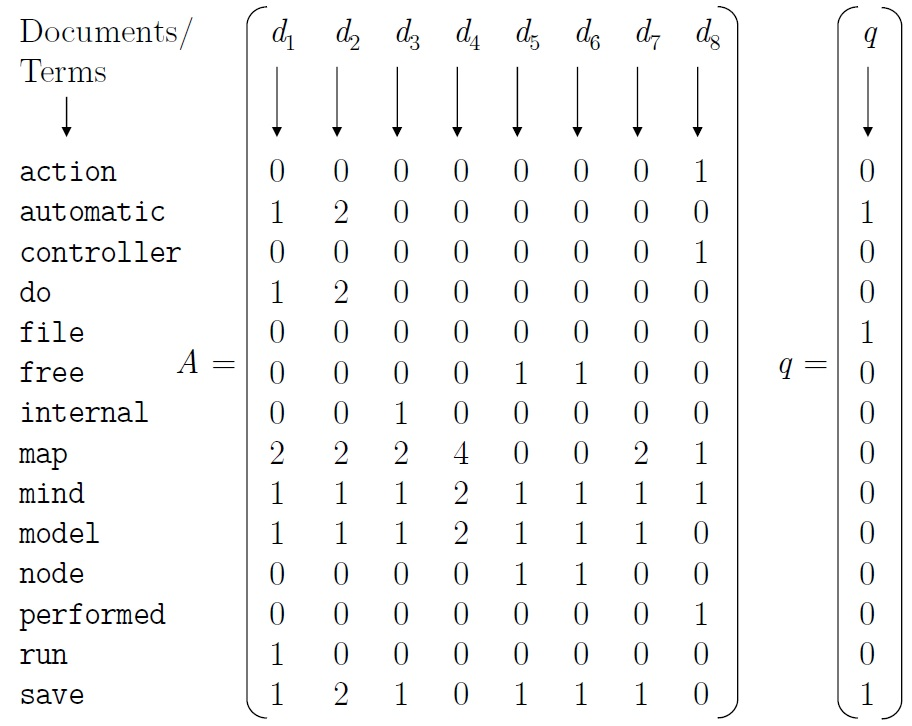
\includegraphics[width=\linewidth]{src/pic/term_document_matrix}
  \caption{The term-document matrix}
  \label{pic:term-document-matrix}
\end{wrapfigure}
The \emph{Latent Semantic Indexing}(short: \emph{LSI}) is an automatic statistical technique. It derives to a given document a vector representation of the query and the corpus by creating a term-document matrix of co-occurring terms. A term $t_i$ is a word, as a tokenized and de-capitalized word of the methods ordered alphabetically and is represented in a row of the matrix. A document $d_j$, which is in the \textit{Freemind-Example} (\autoref{ch:Freemind Example}) a method- or class name, is represented as a column of the matrix. So the matrix, shown in \autoref{pic:term-document-matrix}, looks very similar to the table of FCA (\autoref{table:FCA-finaltable}) with the difference of an unsigned integer value $v_{ij}$, representing how often a document $d_j=MindMapMapModel.doAutomaticSave.run()$ contains token $t_i$, i.e. $d_1$ contains the token $t_7=map$ twice, but the token $t_2=automatic$ only once and does not contain $t_1=action$ at all. Also a query \emph{q} is given, which has a \emph{1} at the terms \emph{automatic}, \emph{save} and \emph{file} representing the feature that should be analysed. 
\begin{wrapfigure}[16]{l}{0.5\textwidth}
  \centering
  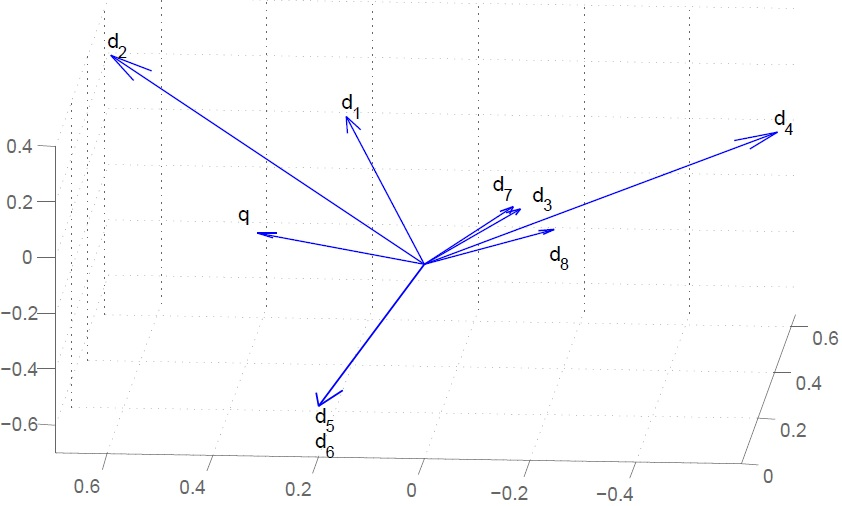
\includegraphics[width=\linewidth]{src/pic/lsf-vectors}
  \label{pic:lsi_vectors}
  \caption{The vector representation of the documents $d_j$ and the query $q$ from the Freemind Example~\ref{ch:Freemind Example}}
\end{wrapfigure}

By normalizing and decomposing using a singular value decomposition the documents can be put into vector representation so that every document has a vector representing their equality to the query $q$. Taking the $cosine()$ of the query $q$ and a document $d_j$ it is possible to measure the similarity. If a document and a query are equal the spreading angle would be $0$ and therefore the best possible similarity is given by $cosine(0)=1$. Also the worst possible angle is $180$, which is equal to document "pointing in the opposite direction", and therefore the worst similarity is given by $cosine(180°)=-1$. We define $cosine(a,b)=\frac{a \cdot b}{||a||*||b||}$ to measure the similarity of two vectors. The common interpretation of the values, regarding that $D$ is the set of all documents, is, that the set-elements $\{d_i \in D| cosine(d_i,q) \ge 0 \} \subseteq D$ are considered to be related to the query of interest, hence every other document is not. It's simple to see that a document is more similar if it points in the same general direction as the query, because of the shared terms. In the Freemind Example the document $d_2=\color{red}MindMapMapModel\color{black}.\color{red}do\color{green}AutomaticSave\color{black}.\color{red}do\color{green}AutomaticSave\color{black}$ is the most similar to the query $q=\color{green}automaticSaveFile\color{black}$, while $d_8=\color{red}MindMapController\color{black}.\color{red}actionPerformed\color{black}$ is the least similar.
\begin{center}
  \begin{tabular}{ c c c c c c c c }
    \hline
    $d_1$ & $d_2$ & $d_3$ & $d_4$ & $d_5$ & $d_6$ & $d_7$ & $d_8$ \\ \hline
    0.6319 & 0.8897 & -0.2034 & -0.5491 & 0.2099 & 0.2099 & -0.1739 & -0.6852 \\ \hline
  \end{tabular}
  \label{table:lsi-values}
\end{center}
Like previously mentioned $d_2$ is the most similar to $q$, because of the "pointing in the same general direction", which it now proven by having the highest value $cosine(d_2,q)=0.8897=max \{ cosine(d_i,q) | d_i \in D \} $ and also $d_8$ is the least similar with a value $cosine(d_8,q)=-0.6852=min\{cosine(d_i,q) | d_i \in D\}$.
  
\section{Term Frequency - Inverse Document Frequency (tf-idf)}
\label{sec:tf-idf}
The \emph{term frequency - inverse document frequency} technique is a statistical technique to derive a feature to a given intension. It measures the importance of a term or multiple terms to documents by its frequency of appearing. The terms are terms of the intension of the feature that is wanted to be analyzed. In a simple way it can be described as: "the more frequent a term occurs in the document, the more relevant the document is to the term". \newline
This is mathematically described as the $document frequency$ $tf=(t,d)$, counting how often the term $t$ is contained in the document $d$.
In the \textit{Freemind-Example} (\autoref{ch:Freemind Example}) the term $t_2 = save$ appears in $d_3$ once and the term $t_1 = automatic$ does not appear at all so: $tf(t_2,d_3) = 1$ and $tf(t_1,d_3)=0$. \newline
Doing that for the terms $t_1 = automatic, t_2 = save$ and $t_3 = file$ and the documents $d_1$ to $d_8$ the matrix shown in \autoref{pic:term-document-matrix} can be derived.
The main problem of this technique is, that uninformative terms appearing within a document-set, often referred as \emph{corpus} and shortened by $D$, maybe even multiple times can distract from terms, which are mentioned less frequent but are more relevant. To compensate that, the technique relativizes by calculating how many documents contain the term and normalizing it. If it's a commonly used term shared by many documents this term can not be taken as a measurement to differentiate between documents. Or colloquially "the more documents include a term, the less this term discriminates between documents ". \newline
So the so-called \emph{inverse document frequency (idf(t))} is calculated as
\begin{center} $idf(t) = log((|D|)/|\{ d \in D | t \in d \}|)$  \end{center}
with $D$ still being the set of documents. And the final \emph{term frequency - inverse document frequency} is the multiplication of both scores, so:
\begin{center} \emph{tf-idf}$(t,d) = tf(t,d) * idf(t)$\end{center}
Regarding the \textit{Freemind-Example} (\autoref{ch:Freemind Example}) the $idf$ terms can be computed as:

\begin{table}[h]
  \centering
  \begin{tabular}{l}
    $t_1 = log(automatic / idf(t_1)) = log(8/2)$  \\
    $t_2 = log(save / idf(t_2))=log(8/6)$ \\
    $t_3 = idf(t_3)=0$ 
 \end{tabular}
\end{table}

Like in the example if the focus is not on one term but on a set of terms the \emph{tf-idf(t,d)} values to a document $d$ are added up. So finally the matrix can be derived as it is shown in Table \ref{table:tfidf_table}.

\begin{table}[h]
  \centering
  \begin{tabular}{| l | c | c | c | c | c | c | c | c |}
    \hline
    & $d_1$ & $d_2$ & $d_3$ & $d_4$ & $d_5$ & $d_6$ & $d_7$ & $d_8$ \\ \hline
    $t_1 = automatic$ & 0.6021 & 1.2041 & 0 & 0 & 0 & 0 & 0 & 0 \\ \hline
    $t_2 = save$ & 0.1249 & 0.2499 & 0.1249 &0 & 0.1249 & 0.1249 & 0.1249 & 0 \\ \hline
    $t_3 = file $ & 0 & 0 & 0 & 0 & 0 & 0 & 0 & 0 \\ \hline \hline
    $\sum\nolimits_{i=1}^3$\emph{tf-idf}$(t_i,d_j)$ & 0.727 & 1.454 & 0.1249 & 0 & 0.1249 & 0.1249 & 0.1249 & 0\\ \hline
  \end{tabular}
  \caption{Term Frequency - Inverse Document Frequency}
  \label{table:tfidf_table}
\end{table}

\section{Hyperlink Induced Topic Search (HITS)}
\label{sec:HITS}
The \emph{Hyper Link Induced Topic Search} (short: \emph{HITS}) is a page ranking algorithm for web mining\footnote{web mining is the analysis step of the knowledge discovery in databases process within the World Wide Web CITE}, which is the counterpart of the famous \emph{Google Page Rank}-algorithm and is currently used by the \emph{Ask Search Engine} \cite{wiki:HITS}. It's basically used to get websites that correspond best to a given input, like every search engine. 
The \emph{HITS}-algorithm distinguishes between two forms of web pages, which are not necessarily disjoint:
\begin{enumerate}
  \item hub \newline
  A hub is a web page pointing towards other web pages , which can be a hub, an authority or even both. A pragmatism is to say: "a good hub points to many authorities."
  \item authority \newline
  An authority is a web page, that other pages point to in order to cite or prove. The rule of thumb is: "a good authority is pointed by many good hubs."
\end{enumerate}

Regarding the definition of hubs and authorities it seems quite natural to define a directed graph $G=(V,E)$ with vertices $V$ = web pages and edges $E = \{(v,w) | v \textrm{ refers to }w\}$ (also called \emph{links}) .
A hubscore is the number of authorities the hub refers to. An authorityscore is a number of good links that refer towards this authority. Both are initialized with 1.
Keeping the graph $G$ in mind the hub- and authority scores can be defined as the following. \newline
\begin{center}
  \begin{tabular}{ r c l }
    authority score of page $p$ & & $A_p= \sum\nolimits_{\{ q | (q,p) \in E \} } H_q $ \\
    hub score of page $p$ & & $H_p = \sum\nolimits_{\{ q | (p,q) \in E \} } A_q $ \\
  \end{tabular}
\end{center}
Given the two values the graph can be rewritten as $G'=(V',E')$ with $V'=\{ (p, H_p, A_p)| \forall p\in V\}$ and $E' = E$.
By iterating over the graph the values of $H_p$ and $A_p$ are calculated for every page $p$. Without any kind of normalization the scores of the adjacent nodes would add up in every iteration leading towards resulting scores that are great but not meaningful numbers. Therefore the normalized score can be computed as the following:
\begin{center}
  \begin{tabular}{ r c l }
    normalizing the authority score of page $p$ & & $A_p= A_p/\sqrt{\sum\nolimits_{ (q,H_q,A_q) \in V' } A_q^2}$ \\
    normalizing the hub score of page $p$ & & $H_p = H_p/\sqrt{\sum\nolimits_{\{(q,H_q,A_q) \} \in V'} H_q^2}$ \\
  \end{tabular}
\end{center}
The normalized values satisfy the condition, that \newline 
\begin{center}
	\vspace{-2em}
	$\sum\nolimits_{\{(p,H_p,A_p) \} \in V'} H_p^2 = \sum\nolimits_{\{(p,H_p,A_p) \} \in V'} A_p^2 = 1$.
\end{center}
\newpage

\begin{wrapfigure}[18]{h}{0.5\linewidth}
  \begin{tikzpicture}
	  \tikzset{vertex/.style = {shape=ellipse,draw,minimum size=3em}}
	  \tikzset{edge/.style = {->,> = latex'}}
	  % vertices
	  \node[vertex] (p1) at  (1,4) {($p_1$, 1, 0)};
	  \node[vertex] (p2) at  (5,2) {($p_2$, 0, 1)};
	  \node[vertex] (p3) at  (1,2) {($p_3$, 1, 2)};
	  \node[vertex] (p4) at  (5,0) {($p_4$, 1, 2)};
	  \node[vertex] (p5) at (-1,0)  {($p_5$, 1, 1)};
	  \node[vertex] (p6) at (-1,-2) {($p_6$, 0, 1)};
	  \node[vertex] (p7) at (2,0)  {($p_7$, 2, 1)};
	  \node[vertex] (p8) at (2,-2) {($p_8$, 2, 0)};
	  %edges
	  \draw[edge] (p1)  to (p3);
	  \draw[edge] (p4)  to (p2);
	  \draw[edge] (p7)  to (p3);
	  \draw[edge] (p3)  to (p5);
	  \draw[edge] (p5)  to (p6);
	  \draw[edge] (p7)  to (p4);
	  \draw[edge] (p8)  to (p4);
	  \draw[edge] (p8)  to (p7);
  \end{tikzpicture}
  \caption{The graph G after the first iteration without normalizing}
  \label{graph:HITS - before first interation}
\end{wrapfigure}

Applying the \emph{HITS}-algorithm to program code hubs can be colloquially described as methods, that call many other methods, and authority's can be described as methods, that implement a function.\newline
In the \textit{Freemind-Example} (\autoref{ch:Freemind Example}) the first graph will look very similar to the class diagram, as it is shown in \autoref{graph:HITS - before first interation}. Keeping the labeling of classes in mind, which was a mapping to the numbers $\#1-\#8$ as it is shown in \autoref{pic:freemind callgraph}, the mapping of the \textit{HITS}-Algorithm is referring to the class \#i as page $p_i$.
After transfering it into the graph of the form of $G'$ and after the first iteration the graph looks like \autoref{graph:HITS - before first interation}. \newline \newline  
Including the normalization the graph $G'$ looks like \autoref{graph:HITS - after first iteration}
The normalization was done by calculating for every $H_p$ and $A_p$ of a page $p$ as:\newline
\begin{center}
  	\vspace{-2em}
  	\begin{tabular}{ r c l }
  		$H_p$ & = &$H_p / \sqrt{1^2+0^2+1^2+1^2+1^2+2^2+0^2+2^2} = H_p/ \sqrt{12}$ and \\
  		$A_p$ & = &$ A_p / \sqrt{0^2+1^2+2^2+2^2+1^2+1^2+1^2+0^2} = A_p/ \sqrt{12}$. \\
	\end{tabular}
\end{center} 

\begin{figure}[h]
	\centering
	\begin{tikzpicture}
		\tikzset{vertex/.style = {shape=ellipse,draw,minimum size=3em}}
		\tikzset{edge/.style = {->,> = latex'}}
		% vertices
		\node[vertex] (p1) at  (1,4) {($p_1$, $\frac{1}{\sqrt12}$, 0)};
		\node[vertex] (p2) at  (6,2) {($p_2$, $\frac{1}{\sqrt12}$)};
		\node[vertex] (p3) at  (1,2) {($p_3$, $\frac{1}{\sqrt12}$, $\frac{2}{\sqrt12}$)};
		\node[vertex] (p4) at  (6,0) {($p_4$, $\frac{1}{\sqrt12}$, $\frac{2}{\sqrt12}$)};
		\node[vertex] (p5) at (-2,0)  {($p_5$, $\frac{1}{\sqrt12}$, $\frac{1}{\sqrt12}$)};
		\node[vertex] (p6) at (-2,-2) {($p_6$, 0, $\frac{1}{\sqrt12}$)};
		\node[vertex] (p7) at (2,0)  {($p_7$, $\frac{2}{\sqrt12}$, $\frac{1}{\sqrt12}$)};
		\node[vertex] (p8) at (2,-2) {($p_8$, $\frac{2}{\sqrt12}$, 0)};
		%edges
		\draw[edge] (p1)  to (p3);
		\draw[edge] (p4)  to (p2);
		\draw[edge] (p7)  to (p3);
		\draw[edge] (p3)  to (p5);
		\draw[edge] (p5)  to (p6);
		\draw[edge] (p7)  to (p4);
		\draw[edge] (p8)  to (p4);
		\draw[edge] (p8)  to (p7);
	\end{tikzpicture}
	\caption{The graph G' after normalizing the hub- and authorityscores}
	\label{graph:HITS - after first iteration}
\end{figure}
\newpage


The final HITS-Graph can be derived as the HITS-graph G from \autoref{graph:HITS - before first interation} iterating for 12 times. In this example after the 12th iteration the values of the pages will not change. The resulting graph is shown in \autoref{graph:HITS - after 100 iterations}. The threshold to consider if a page is relevant or not is in most cases a weighted sum of the hub- and authority score. The common way to interpret the scores is by saying, that pages with high authorityscores implement feature related functions and high hubscores coordinate feature implementing functions.
\begin{figure}[h]
	\centering
	\begin{tikzpicture}
	\tikzset{vertex/.style = {shape=ellipse,draw,minimum size=3em}}
	\tikzset{edge/.style = {->,> = latex'}}
	% vertices
	\node[vertex] (p1) at  (1,4) {($p_1$, 0.328, 0)};
	\node[vertex] (p2) at  (8,2) {($p_2$, 0, 0)};
	\node[vertex] (p3) at  (1,2) {($p_3$, 0, 0.591)};
	\node[vertex] (p4) at  (8,0) {($p_4$, 0, 0.737)};
	\node[vertex] (p5) at  (-2,0) {($p_5$, 0, 0)};
	\node[vertex] (p6) at  (-2,-2) {($p_6$, 0, 0)};
	\node[vertex] (p7) at  (3,0) {($p_7$, 0.737, 0.328)};
	\node[vertex] (p8) at  (3,-2) {($p_8$, 0.591, 0)};
	%edges
	\draw[edge] (p1)  to (p3);
	\draw[edge] (p4)  to (p2);
	\draw[edge] (p7)  to (p3);
	\draw[edge] (p3)  to (p5);
	\draw[edge] (p5)  to (p6);
	\draw[edge] (p7)  to (p4);
	\draw[edge] (p8)  to (p4);
	\draw[edge] (p8)  to (p7);
	\end{tikzpicture}
	\caption{G' after 12 iteration steps and only in the last step rounded values}
	\label{graph:HITS - after 100 iterations}
\end{figure}

The resulting graph in \autoref{graph:HITS - after 100 iterations}, can be interpreted by a function:
\begin{center}
	$f(v) = \begin{cases} 1 \qquad ,if \ v_h>0.7\\ 1 \qquad ,if \ v_a > 0.4 \\ 0 \qquad else \end{cases}$
\end{center}
The result $f(v)=1$ is considered relevant, with  $v\in V$ and $v_h, v_a$ being the corresponding hub-/authorityscores. Therefore the method will consider $p_3$ and $p_4$ as relevant, which is only 50\% of the pages that should be relevant as stated in \autoref{ch:Freemind Example}. The other two relevant pages $p_1$ and $p_2$ are not considered, so called \emph{false-negatives}, because of their appearance within the callgraph. $p_1$ has a very low hubscore and no authority value and $p_2$ no value at all. So the \emph{HITS-Algorithm} does not work quite well on this example because of the callgraph structure, but combining it with other techniques leads to the fact that the \emph{HITS-Algorithm} is a frequently used technique.
%\clearpage


\chapter{Classification and Methodology}
\label{ch:Classification and Methodology}
%\section{Eins - Eins}
%\subsection{Eins - Eins - Eins}

% Die Logos sind veraltet und duerfen zurzeit nicht verwendet werden!
% Auf Seite \pageref{Logo} in Abbildung \ref{Logo} befindet sich das SE Logo.
The classification of feature location techniques is very important, because of the different special demands of some classes of techniques and their assumptions they have towards special parts of the system or code.
The first big distinction is the difference of dynamic and static techniques. \newline
\\
\underline{dynamic}:\newline
Dynamic approaches collect information about the program at runtime. They do so by using program dependency analysis, information retrieval, latent semantic indexing (\autoref{sec:LSI}) or the term frequency - inverse document frequency {(\autoref{sec:tf-idf}), only considering the methods and classes, which are involved during the current execution of the program. This is a big advantage, because by knowing roughly the part of the program where it could be used the user is able to steer the program into the direction. In our example the \emph{automaticSaveFile}-function would not be in the main-menu or the settings, but is more likely to be involved if the user creates a mind map and waits till the \emph{automaticSaveFile}-function is triggered. But that advantage has also it's downside. By only analysing the involved parts of the program the whole information retrieval is based on the input the program gets and has to generalize from that, which contains the possibility of leaving out important parts not considered during the scenarios. Also collecting information on test-cases can only derive \emph{functional} requirements, but is not able to derive non-functional requirements. In general the dynamic approaches under approximate, because of the lack of possibility to derive every requirement the and the generalizing without in depth detailed information.\newline
\underline{static}:\newline
Static approaches do not need the program to be executed. They collect information directly out of the source, which has  one big disadvantage. A static approach would look at every single part of the code to derive information about the feature, the user wants to locate, which can be very costly. Imagine a program which is very complex and contains thousands of lines code within hundreds of classes and the user wants to locate a very small special feature which is contained in very little of the code for example in only 0.01\% . The static approach will look through the whole 100\% of code, of which 99.99\% are not related to the feature. The big advantage of the static approach is that the information it reveals are safe, which means it does not has to generalize out of a case but can validate on the whole information. This results in the ability to derive functional and non-functional requirements. This whole information can on the other side lead again to problems. Knowing every little detail can lead to situations in which the information's are undecidable in the matter of affiliation to the feature. So the technique has to approximate a solution, which may be to imprecise. In general the static approaches over approximate. \newline
\\
The techniques can also be splitted within the \emph{static}/\emph{dynamic}-groups due to the form of output the methods give. \newline \\
\underline{plain}:\newline
The plain-output techniques present an unsorted list of artefacts, which are considered by the technique to be relevant to the feature. They leave the interpreting of the output to the user. \newline
\underline{guided}:\newline
The guided-output techniques present the collected artefacts in a special arrangement to build an interpretation, like ordering the artefacts based on the relevance it is considered to have. Also often a so called \emph{Program Dependency Graph} is given to not only show relevant artefacts, but also give a dependency of these artefacts. This topic is further explained in "Case Study of Feature Location Using Dependence Graph" by K. Chen and V. Rajlich \cite{chen2000case}.\newline

Also the different techniques make assumptions. For example \emph{Latent Semantic Indexing}, which is explained in \autoref{sec:LSI}, does the assumption that the classes and methods of the code are named like the function they implement. The same technique can be useful on one code fragment, which fits the assumptions, but completely useless on an other one, which does not fulfil the assumptions \cite{rubin2013survey} \cite{dit2013feature}. \newline

Another file in which the different methods can be distinguished is the amount of user interaction within the process of locating a feature. While some methods can derive features and corresponding artefacts with almost only the name of the wanted feature, others need very much interaction to derive these artefacts The result depends on the underlying code, the feature and also on the assumptions they make towards the code.\newline
%\clearpage

\chapter{Feature Location Techniques}
\label{ch:feature location techniques}
%\section{Eins - Eins}
%\subsection{Eins - Eins - Eins}

% Die Logos sind veraltet und duerfen zurzeit nicht verwendet werden!
% Auf Seite \pageref{Logo} in Abbildung \ref{Logo} befindet sich das SE Logo.
In this chapter deals with five different feature location techniques in detail. They are defined as two static and two dynamic techniques with each one technique giving plain, one giving guided output and the static plain technique \emph{SNAIFL} as a special case. The techniques presented in the following can be classified by the characteristics of \autoref{ch:Classification and Methodology}:

\begin{table}[h]
	\begin{tabular}{|l| l l l l l l|}
		\hline
		 & technique &  output & underlying & input & result & user \\ 
		 &  &  &  technology &  &  &  \\ \hline
		 \multirow{5}{1em}{\begin{sideways} static \end{sideways}}
		 & Find-concept  & plain & PDA, NLP & query & AOIG & ++  \\
		 &      &        &             & query         & documents  &   \\
		 & SNIAFL & plain & tf-idf, LSI, & set of query's & BRCG & -/+ \\ 
		 &        &       & PDA  &             &      &
		 \\ 
		 & Dora & guided & PDA, tf-idf & method, depth & call graph & + \\ 
		 &      &        &             & query         & documents  &   \\ \hline
		 \multirow{4}{1em}{\begin{sideways} dynamic \end{sideways}}
		 & Software & plain & FCA, PDA & set of & executable & +++ \\ 
		 & Reconnaissance &  &  & scenarios, query & & \\
		 & Revelle  & guided & trace analysis & scenario and & executable, & +\\
		 &   &  & LSI, HITS & query & documents & \\ \hline
		
	\end{tabular}
	\caption{The techniques discussed further on in this paper}
	\label{table:techniques overview}
\end{table}

\section{Static - Plain}
\label{sec:find-concept}
As an example of a static technique with plain output the \emph{Find-concept (short FC)} of David Shepherd, Emily Hill, K. Vijay-Shanker and Lori Pollock of the University of Delaware and also Martin P. Robillard of the McGill University in Canada is a reasonable choice \cite{shepherd2007using}.
The technique makes, as previously mentioned in \autoref{ch:Classification and Methodology}, some assumptions to the underlying code. To apply \emph{FC} the code has to be object-oriented, the comments and identifiers, which are objects and methods, have to be named in a way so that the technique can retrieve domain knowledge. Also it makes the premise that verbs correspond to methods and nouns refer to objects. Also FC defines so called \textit{direct objects}, which are objects corresponding to a verb. In our example the verb $save$ corresponds to $MindMapMapModel$, $MindMapNodeModel$ and $MindMapEdgeModel$, which are therefore the direct objects of $save$.\newline
\emptyLine
The input to the FC is given by the user as a query of description phrases of the feature of interest and after that decomposed into a set of \textit{verb-DO} pairs. In order to improve the result the technique collects related words, like synonyms or verbs in different time forms, and also regards words, which are often mentioned in the context of words from the query. These collected words then get ranked by their similarity to the query words using LSI (\autoref{sec:LSI}), calculating with a variable weight for the synonyms, and the ten most analogous are presented to the user to augment the query with these terms and program methods already matching to the current query.\newline
\emptyLine
The important aspect the user wants to retrieve are the \textit{verb-DO} pairs matching the query. To be able to derive the matching pairs the FC builds an \textit{action-oriented identifier graph model (AOIG)}. The \textit{AOIG} contains four kinds of nodes and 2 types of edges:
%\vspace{3em} %WARNING: may be shitty

\begin{table}[th]
	\begin{tabular}{r l}
		\textit{verb nodes}: & a node for each specific verb/action \\
		\textit{direct object (DO) nodes}: & a node for each direct object \\
		\textit{verb-DO nodes}: & a node for every \textit{verb-Do} pair. \\
		&(A \textit{DO} can be in multiple \textit{verb-DO} nodes) \\
		\textit{use nodes}: & a node for each incidence of a \textit{verb-DO} pair in comments \\
		& or the source code \\
		 & \\
		\textit{pairing edges}: & connecting every verb and DO to the \textit{verb-DO nodes} \\
		&containing them \\
		\textit{use edges}: & connecting each \textit{verb-DO node} to every corresponding \\
		& \textit{use node}.
	\end{tabular}
\end{table}

After several steps of improving the query the final query traverses through the \textit{AOIG} and filters every \textit{verb-DO} pair containing words of the query, extracting all methods using the filtered pairs and apply \textit{Program Dependency Analysis (PDA)} on it to reveal call relations within the extraction.

Finally the \emph{FC} is able to generate the result graph with methods matching the query as nodes and structural relations between the methods computed by the \textit{PDA}. \cite{shepherd2007using} \newline
Due to the overhead of computing the \textit{verb-DO} pairs out of the query and the step by step improvement of the input the user interaction in Table \ref{table:techniques overview} is rated with "++".

\section{Static - Guided}
\label{sec:Dora}
The technique presented by \emph{Emily Hill, Lori Pollock} and \emph{K. Vijay-Shanker}, professors of the \textit{University of Delaware} in  \textit{Computer and Information Science}, is named \emph{Dora the Program Explorer} (short: \emph{Dora}})\footnote{Dora comes from exploradora, the Spanish word for a female explorer\cite{hill2007exploring}. Also the name chosen in account of the children's series "\textit{Dora the Explorer}" }\cite{hill2007exploring}.
Dora also uses a call graph $G=(V,E)$ to derive dependency, like the \emph{Find-concept} in \autoref{sec:find-concept}, but combines it with the \emph{tf-idf} ranking method explained in \autoref{sec:tf-idf} with the methods as nodes $n \in V$, it's body as the documents $d(n)$ and edges $e=(n,m) \in E$ if $n$ calls $m$. \newline
As an input the user has to yield an initial query, a so called \textit{seed method} $ n_0 \in V$ the examination should start from, and a depth defining a graph-neighbourhood, which should be included in the search(i.e. a maximal distance). \newline
Given the input, Dora proceeds by traversing through the call graph $G$ calculating how suitable the document $d(n)$ of the current node $n$ is by combining the succeeding three values:
\begin{enumerate}
	\item the \emph{tf-idf} score of the identifiers within the method name ($n$)
	\item the \emph{tf-idf} score of the identifiers within the method body ($d(n)$)
	\item a binary value to indicate if the method belongs to a library or is part of the user-made code
\end{enumerate}
Dora can be parametrized by the weight of these three components, for example the method name(1) should be more important than the method body(2) and if the method is out of a library it should not be considered, which leads to the following formulae:
\begin{center}
	$\quad s(n)= (1-b) * [ \frac{2}{3} $\emph{tf-idf}$(n) + \frac{1}{3}$\emph{tf-idf}$(d(n)) ]$
\end{center} 
where $b$ defines if $n$ belongs to a library($b=1$) or $n$ is user-made($b=0$).
There are two more adjustable values: the relevance threshold($rt$) and exploration threshold($et$). The relevance threshold determine whether a node is relevant or not can be parametrized by giving a value $rt,et \in [0,1] $ and typically $et < rt$, that given a node $n$:
\vspace{2em} %WARNING: might be shitty
\begin{table}[h]
	\centering
	\begin{tabular}{r c l}
		$rt <= s(n)$ & $\rightarrow$ & the node is relevant\\
		$et <= s(n) < rt$ & $\rightarrow$ & the node is not relevant, but maybe it's neighbours \\
		$s(n) < et$ & $\rightarrow$ & the node can be neglected
	\end{tabular}
\end{table}

In the case of 1 and 2 Dora traverses to the neighbourhood of the node, if it does not harm the initial depth, and otherwise discards the node. So in finite steps of traversing through the call graph Dora has reached a point, where no additional elements need to be explored.\newline
The result Dora computes is a subgraph $G'=(V',E')$ of the call graph, where $V' = \{ n \in V | et <= s(n) \}$, $E' = \{ (n,m) \in E | n,m \in V' \}$ and a function \newline
\[
	f: n\in V' \rightarrow \{0,1\},n \rightarrow 
		\left\{
			\begin{array}{ll} 
				1, & s(n) >= rt \\
				0, & else 
			\end{array}\right. .
\]
This function can be described as a colouring of every \textit{relevant} node. The final output is the coloured sub-call-graph $G'$. \newline
\emptyLine
In the \textit{Freemind Example} of \autoref{ch:Freemind Example} the result can look different, by changing the parameters like the \textit{seed method}, the \textit{depth} or the \textit{threshold values}.
Simplifying the method in the fact of disregarding the method body's and by knowing that every method called in the \autoref{pic:freemind callgraph} is user made, the scores are equal to their score in \autoref{table:tfidf_table}. \newline
The threshold are chosen like the following:
\begin{table}[h]
	\centering
	\begin{tabular}{r l}
		$rt = 0.5$ & methods with a score of 0.5 or higher are considered relevant \\
		$et = 0.1$ & methods with a score of 0.1 or higher should be explored further
	\end{tabular}
\end{table}
So the final graph Dora computes looks like the \autoref{graph:Dora - result}. The green nodes are relevant to the feature, the grey nodes are explored but not relevant. The red node(\#2) is highly relevant to the feature with a \emph{tf-idf score} of 1.454, but is not explored due to the \textit{depth} of 3.
\begin{figure}[h]
	\centering
	\begin{tikzpicture}
		\tikzset{vertex/.style = {shape=ellipse,draw,minimum size=1.5em}}
		\tikzset{edge/.style = {->,> = latex'}}
		% vertices
		\node[vertex, fill=black!30!green] (p1) at  (0,2) {\#1};
		\node[vertex, fill=black!30!red] (p2) at  (3,2) {\#2};
		\node[vertex, fill=gray] (p3) at  (0,0) {\#3};
		\node[vertex, fill=gray] (p4) at  (3,0) {\#4};
		\node[vertex, fill=gray] (p5) at (-1,-1)  {\#5};
		\node[vertex, fill=gray] (p6) at (-1,-2.5) {\#6};
		\node[vertex, fill=gray] (p7) at (1,-1)  {\#7};
		\node[vertex, fill=gray] (p8) at (1,-2.5) {\#8};
		%edges
		\draw[edge] (p1)  to (p3);
		\draw[edge] (p4)  to (p2);
		\draw[edge] (p7)  to (p3);
		\draw[edge] (p3)  to (p5);
		\draw[edge] (p5)  to (p6);
		\draw[edge] (p7)  to (p4);
		\draw[edge] (p8)  to (p4);
		\draw[edge] (p8)  to (p7);
	\end{tikzpicture}
	\caption{The result graph of \textit{Dora}, with \#1 as \textit{seed method}, \textit{depth}=3, rt=0.5 and et=0.1}
	\label{graph:Dora - result}
\end{figure}
 In modern cases of application the \textit{threshold}-values are chosen by a heuristic of other cases and general knowledge of the underlying program. Including the \textit{methods body} (2) and the binary value of the formulae the result can be refined by slightly changing the query or the \textit{threshold's}. \newline
\emph{Dora} only needs a query and a \textit{depth} to compute a result, which takes to further interaction, which is marked within the \autoref{table:techniques overview} with only one "+".

\section{Dynamic - Plain}
\label{sec:Wilde}
One of the most important dynamic plain approaches is the very first one of Norman Wilde and Michael Scully known under the term \emph{Software Reconnaissance} \cite{wilde1995software}. \textit{Software Reconnaissance} tries to define a feature $f$ by getting two sets of scenarios $S_f$ and $\overline{S_f}$ as an input and distinguishing between scenarios that invoke the feature of interest $S$ and scenarios that do not $\overline{S_f}$. \newline
Regarding the execution traces \textit{Software Reconnaissance} categorizes methods/lines of code $M$\footnote{the degree of fineness is chosen by the user} into three groups:
\begin{table}[h]
	\begin{tabular}{l}
		1. potentially involved  \\
 		\qquad $I_1 = \{ m \in M | \exists s \in S_f$ s.t. $s$ executes $m \}$ \\
 		\qquad get executed by \underline{at least one} scenario of $S_f$\\
		2. indispensably involved  \\
		\qquad $I_2 = \{ m \in M | \forall s \in S_f : s$ executes $m \}$ \\
		\qquad get executed by \underline{every} scenario of $S_f$\\
		3. uniquely involved  \\
		\qquad $I_3 = \{ m \in M | m \in I_1$ and $\forall s\in \overline{S_f} : s$ does \underline{not} execute $m \}$ \\
		\qquad executed by at least one scenario of $S_f$ and by no scenario of any other feature\\
		4. common components  \\
		\qquad $C = \{ m \in M | \forall s \in S_f \cup \overline{S_f}:s$ executes $m \}$ \\
		\qquad used by every scenario (for example a \textit{main}-method)
	\end{tabular}
\end{table}
The result are the first 3 lists for every feature $f$ that is set in the query and once the list of all \textit{common} components. Different versions of this technique state, that $I_2 \cap C = \emptyset$.\cite{wilde1995software} \newline
\emptyLine
In our example regarding the two features of $f_1 = automaticSaveFile$ and $f_2 = manualSaveFile$ the execution traces are quite similar owed to the fact, that the \textit{automaticSaveFile}-feature is just a not user triggered \textit{internalSave}. Keeping in mind the call graph(\autoref{pic:freemind callgraph}) methods \#3, \#5 and \#6 will be considered as \textit{common} components. Method \#1 will be considered \textit{uniquely involved} to the feature $f_1$. \newline
\emptyLine
This technique already requires voluminous overhead, because of the two sets of scenarios $S_f$ and $\overline{S_f}$ for every feature.


\section{Dynamic - Guided}
\label{sec:Revelle}
The dynamic guided technique by Meghan Revelle, Bogdan Dit and Denys Poshyvanyk, which are professors at the College of William and Mary in Virginia, is based on a chain of other techniques here and further named as the main author:
\begin{center}
	$Revelle \cite{revelle2010using} \rightarrow Liu \cite{liu2007feature} \rightarrow Poshyvanyk \cite{poshyvanyk2007feature} \rightarrow Marcus \cite{marcus2004semantic}$
\end{center}
The very base technique by Marcus is to take a given input query and convert it into a document in vector space using the in \autoref{sec:LSI} mentioned \textit{LSI}. The technique then separates different software elements, for example methods, and creates separate documents using the identifiers and also converting them into vector space. The identifiers are often separated using typical code style, like the connecting of two words using "\underline{ }" or changing from lower to upper case letters. In order to filter the result the search space in partitioned by refining the documents similarity values, so that in step $i+1$ are only the documents of step $i$, which are higher than a given threshold. After that the user decides which documents are relevant to the feature. Once the user decides that no further document is relevant to the feature the the algorithm terminates. \cite{marcus2004semantic} \newline
%In addition to \textit{Marcus} \textit{Poshyvanyk} uses FCA \autoref{sec:FCA} to rank the documents after they are ranked on the similarity to the input query. \textit{Poshyvanyk} takes the first $n$ documents and ranks the \emph{uniquely} appearing terms in the documents based on the similarity the term and the corpus-document in a way, that terms, which are similar to terms in the $n$ documents but not in the rest, are ranked higher. On the other hand terms, which are similar to documents not being in the top $n$ documents, are penalized because might have identifiers for not relevant things with relevant names and therefore would distort the result. After ranking the unique terms \textit{Poshyvanyk} selects the top $k$ terms as \textit{attributes} out of the top $n$ documents, which are the \textit{objects}, and apply FCA \autoref{sec:FCA}. So the user gets not only the space vectors of the similarity of the documents, but also gets a visualization of the terms used within. \newline
\textit{Poshyvanyk} uses a combination of \textit{Marcus} \textit{LSI} method and \textit{execution-trace analysis} \footnote{further information on that topic within the \textit{IEEE}-paper \cite{antoniol2006feature}}. To analyse a program it has to be given as an input in an executable form, to determine which methods are called on a scenario, and a set of documents, which can be defined out of a query with \textit{Marcus}. Also the technique needs two sets of scenarios: one that invoke the feature of interest and one that does not. First the technique ranks the documents like within \textit{Marcus}. After that the scenario sets are executed and execution profiles are derived. By that the methods can be ranked by the appearance within the traces of the scenarios that execute the feature versus the appearance within the other scenarios. The final result of a method is a weighted sum of the \textit{LSI}-rank and the \textit{trace}-rank. So the final output is the again a ranked list of methods. \cite{poshyvanyk2007feature} \newline
The technique \textit{Liu} is quite similar to \textit{Poshyvanyk}, with the difference, that instead of using two sets of scenarios \textit{Liu} only works with a single scenario executing the feature of interest. This reduces the overhead of input and also accelerates the process, accepting the fact that the result may not be as accurate as it would be with \textit{Poshyvanyk}. \cite{liu2007feature} \newline
The technique \textit{Revelle} combines \textit{Information Retrieval}, \textit{dynamic} and \textit{web-mining} analysis in order to improve the results of the previous methods. Like \textit{Liu} \textit{Revelle} gets a single scenario that exercises the feature of interest and a query as input. While running the scenario the call graph from the execution trace is constructed, which nodes are methods that are actually executed. Every node gets a score using a web-mining algorithm like the HITS-algorithm mentioned in \autoref{sec:HITS}. After assigning the values \textit{Revelle} filters one of the following two out:
\begin{itemize}
	\item low-ranked methods 
	\begin{itemize}
		\item typically used on \textit{HITS authority score}
		\item methods that are not called often are not extremely important
	\end{itemize}
	\item high-ranked methods 
	\begin{itemize}
		\item typically used on \textit{HITS hub score}
		\item  methods that call very many other methods are not meaningful
	\end{itemize}
\end{itemize} 
The remaining set of methods get ranked by using \textit{Liu} and the final ranked list is returned to the user.
The overall user interaction is quite sparely, because of one scenario and a query about the feature of interest and therefore rated with "+" in \autoref{table:techniques overview}. \cite{revelle2010using}

\section{Future Technique Approaches}
\label{sec:SNIAFL}
All of the presented techniques are still under research to improve the results accuracy, the runtime and the amount of user interaction. Even if the last point is not that important in the beginning is can be the most essential due to the possibility of high serialisation. Also the generally preferred technique group is the static one, because of the high amount of pre-computing used to derive scenarios and checking if they invoke the feature and the execution time used to run these.\newline
\textit{W. Zhao, L. Zhang, J. Sun and F. Yang} from the University of Peking in cooperation with \textit{L. Yin} of the Rensselaer Polytechnic Institute are working on an approach of a \textit{static non-interactive} technique by using \textit{Program Dependency Analysis} and \textit{Information Retrieval} technologies \cite{zhao2006sniafl}.\newline
They define two types of functions of a feature:
\begin{enumerate}
	\item \textit{specific functions}:
	functions only used to implement the feature and not used by any other feature.
	\item \textit{relevant functions}:
	functions involved in the implementation of the feature
\end{enumerate}
The set of \textit{specific features} is indisputable a subset of the set of \textit{ relevant features}.
The presentation of the program within the technique is realized with a so called \textit{Branch-Reserving Call Graph (BRCG)}, which is a normal call graph expanded with branching and sequential information. These informations can be used to construct pseudo execution traces for a feature. The \textit{BRCG} can be written as $G=(V,E)$ with the nodes $V$ as a function, a branch or a return statement. Loops are defined as two branch statements: one going through the loop body and one exiting immediately.

%\begin{figure}[hbt]{0.5*\textwidth}
%	\lstset{language=Java}
%	\lstinputlisting[
%	label=lst:system,
%	caption=An example code for BRCG] {src/listings/BRCG-examplecode.java}
%\end{figure}

\noindent\begin{minipage}{.35\textwidth}
	\lstset{language=Java}
	\lstinputlisting[
		label=lst:code,
		caption=An example code for BRCG] {src/listings/BRCG-examplecode.java}
\end{minipage}\hfill
\begin{minipage}{.55\textwidth}
%	\begin{tikzpicture}
%		\tikzset{method/.style = {shape=circle,draw,minimum size=3em}}
%		\tikzset{decision/.style = {shape=diamond,draw,minimum size=1em, node distance=3em}}
%		\tikzset{sequential/.style = {shape=rectangle,draw,minimum width=4em,,node distance=2.25em}}
%		\tikzset{branch/.style = {shape=ellipse,draw,minimum width=3em,node distance=3em}}
%		\tikzset{edge/.style = {->,> = latex'}}
%		
%		\node[method] (method) at  (5,1) {func};
%		\node[sequential, below of=method](method_sequential) {sequential};
%		
%		\node[method, below left = of method_sequential] (f1) {f1};
%		\node[decision, below = of method_sequential](BS1){BS1};
%		\node[branch, below of=BS1](BS1_branching) {branching};
%		\node[method, below right = of method_sequential] (f6){f6};
%		
%		\node[method, below left = of BS1_branching] (B1) {B1};
%		\node[sequential, below of=B1](B1_sequential) {sequential};
%		\node[method, below right = of BS1_branching] (B2) {B2};
%		\node[sequential, below of=B2](B2_sequential) {sequential};
%		
%		\node[method, below left = of B1_sequential] (f2) {f2};
%		\node[method, below right = of B1_sequential] (exit) {exit};
%		
%		\node[decision, below left = of B2_sequential] (BS2) {BS2};
%		\node[branch, below of=BS2,node distance=3em](BS2_branching) {branching};
%		\node[method, below right = of B2_sequential] (f5) {f5};
%	\end{tikzpicture}

%	\begin{forest}
%		method/.style = {shape=circle,draw,minimum size=3em},
%		decision/.style = {shape=diamond,draw,minimum size=1em},
%		sequential/.style = {shape=rectangle,draw,minimum width=4em,,node distance=2.25em},
%		branch/.style = {shape=ellipse,draw,minimum width=3em,node distance=3em},
%		edge/.style = {->,> = latex'}
%		[{func},method
%			[{f1}, method],
%			[{BS1}, method],
%			[{f6}, method]
%		]
%	\end{forest}
	\vspace{-5em}
	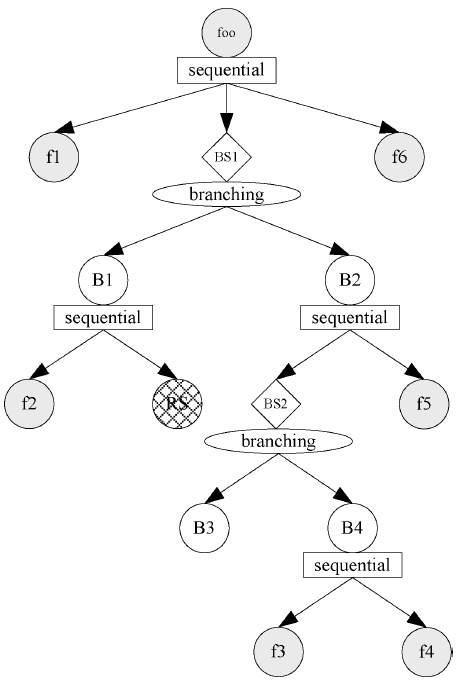
\includegraphics[width=.75\textwidth]{src/pic/BRCG-example.png}
	\captionof{figure}{The BRCG of the example code in \autoref{lst:code} \cite{zhao2006sniafl}}
	\label{graph:BRCG}
	\vspace{2em}
\end{minipage}
In \autoref{graph:BRCG} is shown an example graph for the example code of \autoref{lst:code}, with $f1$ to $f6$ being function. The nodes $func, B1, B2$ and $B4$ are \textit{sequential} of code, which indicate a sequence of other nodes following, while $BS1$ and $BS2$ are \textit{branching} nodes indicating a conditional-based decision, like an if-statement or a \textit{while}-loop. $RS$ is a \textit{return}-statement and $B3$ is the automatic \textit{exit}-statement previously mentioned.\newline
As an input the technique takes textual paragraphs for every feature, which can be derived by the requirements documentation. These paragraphs are converted into documents using the code style  like in \autoref{sec:Wilde} and normalizing\footnote{in general converting to lower case alphabetical letters} the terms. Also \textit{FCA} (\autoref{sec:FCA}) will be used to convert the methods into queries. \newline
After deriving the documents and queries the technique uses a special \textit{LSI} variation to convert these two sets to a vector space and measure the similarity using the $cosine$. The speciality of this variation is, that the weights of the terms, defining which terms are more important than others, are not given by the user or chosen equally balanced, but are also computed using \textit{tf-idf} (\autoref{sec:tf-idf}).\newline
After these steps the technique has a ranked list $L_d$ of queries(functions) for every document $d$ (feature) ranked by their similarity. Within every list is a pair of queries $p$ with the largest difference so $p^d = max\{ (q^d_i, q^d_{(i+1)}) \in L_d | p^d_i - p^d_{(i+1)} \}$, called \textit{division point}. Every function before the \textit{division point} are considered \textit{initial specific functions} to the feature. \newline
The next step is to traverse the \textit{BRCG} and cut off every branch that does not contain any of the \textit{initial specific functions}, considered to be not relevant to the feature. Vice versa every other function is marked as relevant. So a pseudo-execution can be given to the user as a traversing through the trimmed \textit{BRCG}.\newline

Overall the technique is based on a high amount of computation but works without a single input. \textbf{But} in reality the requirements documentation and comments are not enough to generate that much knowledge about the features, that they can be derived satisfyingly. So the technique works on programs that are written in a certain way, which is not the final solution but is an approach leading the way.




%\clearpage


%\chapter{Code Listings}\label{ch:listings}
%% use language 'myLng' for the next listings (until another language is set)
%% include listing 'listings/AdverseReactionApp.aj' with label and caption
%% note: big listings sometimes need to overwrite the float value that has been
%% already set in the general listings setup (see paper.tex)

%This chapter contains the beautiful listing \ref{lst:system}. 
Lorem ipsum dolor sit amet, consetetur sadipscing elitr, sed diam nonumy 
eirmod tempor invidunt ut labore et dolore magna aliquyam erat, sed diam 
voluptua. At vero eos et accusam et justo duo dolores et ea rebum. Stet 
clita kasd gubergren, no sea takimata sanctus est Lorem ipsum dolor sit 
amet. Lorem ipsum dolor sit amet, consetetur sadipscing elitr, sed diam 
nonumy eirmod tempor invidunt ut labore et dolore magna aliquyam erat, 
sed diam voluptua. At vero eos et accusam et justo duo dolores et ea 
rebum. Stet clita kasd gubergren, no sea takimata sanctus est Lorem 
ipsum dolor sit amet. 




\begin{figure}[hbt]
\lstset{language=MontiArc}
\lstinputlisting[
label=lst:system,
caption=Code listing with user defined syntax highlighting (MontiArc).] {src/listings/AdverseReactionApp.aj}
\end{figure}

\cleardoublepage


%\chapter{Conclusion}

In these chapters 4 basic underlying techniques (\autoref{ch:basic underlying techniques}) and a technique for every major category (\autoref{ch:feature location techniques}) are presented, which are only the peak of the iceberg. Given an example of the Freemind Mind mapping software (\autoref{ch:Freemind Example}) and explaining the techniques based on it the general function of feature location techniques are shown. Overall the conclusion of the techniques is an obvious, but not irrelevant statement: \newline
\begin{center}
	No \textit{Feature Location Technique} can be perfect in every kind of scenario, but by knowing the exact fitting assumptions the best resulting technique can be chosen.
\end{center} 

Feature Location Techniques are an essential part of software development and in preparing the steps towards Software Product Line Engineering. Reality shows that even with the best architecture and planning software project tend to be a complex and highly branched construct, which are almost impossible to be analysed without any help of techniques. \newline
The field of Feature Location is not a new upcoming issue, but never the less it is still up-to-date. The growth of software projects keeps increasing and therefore the amount of issues that comes along. Common techniques are still refined and new techniques are developed in a constant manner. New heuristics of weighting are neglecting aspects can change a technique from an average resulting technique to one that has the ability to locate features like no other. But the even best technique is only reliable on a decent fit to its assumptions. \newline



\cleardoublepage


\bibliographystyle{alpha}
\addcontentsline{toc}{chapter}{Literaturverzeichnis}
\bibliography{src/bib/Literatur}

% Begin Anhang
%\appendix
%\chapter{z.\,B. Programmdokumentation}

\cleardoublepage


\end{document}
